\documentclass{standalone}
\usepackage{tikz}
\usetikzlibrary{arrows.meta} % For nicer arrowheads

\begin{document}
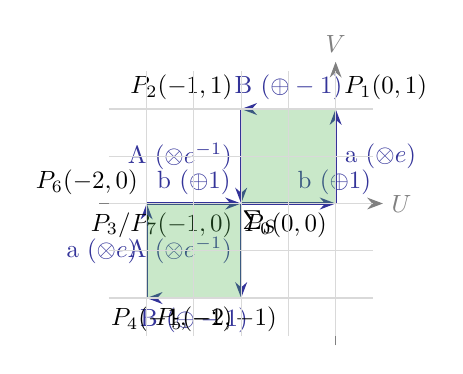
\begin{tikzpicture}[scale=1.2, every node/.style={scale=0.9, auto}]
    % Define coordinates for the path aBAABabb with t=e (ln t = 1)
    \coordinate (P0) at (0,0);      % Start
    \coordinate (P1) at (0,1);      % after a
    \coordinate (P2) at (-1,1);     % after B
    \coordinate (P3) at (-1,0);     % after A
    \coordinate (P4) at (-1,-1);    % after A
    \coordinate (P5) at (-2,-1);    % after B
    \coordinate (P6) at (-2,0);     % after a
    \coordinate (P7) at (-1,0);     % after b (Note: P7 is same as P3)
    \coordinate (P8) at (0,0);      % after b (Note: P8 is same as P0, path closes)

    % Draw path segments with labels for operations
    % Using a slightly darker color for the path itself
    \definecolor{pathcolor}{rgb}{0.2,0.2,0.6}
    \draw[-{Stealth[length=2mm, width=1.5mm]}, thick, pathcolor] (P0) -- (P1) node[midway, right] {a ($\otimes e$)};
    \draw[-{Stealth[length=2mm, width=1.5mm]}, thick, pathcolor] (P1) -- (P2) node[midway, above] {B ($\oplus -1$)};
    \draw[-{Stealth[length=2mm, width=1.5mm]}, thick, pathcolor] (P2) -- (P3) node[midway, left]  {A ($\otimes e^{-1}$)};
    \draw[-{Stealth[length=2mm, width=1.5mm]}, thick, pathcolor] (P3) -- (P4) node[midway, left]  {A ($\otimes e^{-1}$)};
    \draw[-{Stealth[length=2mm, width=1.5mm]}, thick, pathcolor] (P4) -- (P5) node[midway, below] {B ($\oplus -1$)};
    \draw[-{Stealth[length=2mm, width=1.5mm]}, thick, pathcolor] (P5) -- (P6) node[midway, left]  {a ($\otimes e$)};
    \draw[-{Stealth[length=2mm, width=1.5mm]}, thick, pathcolor] (P6) -- (P7) node[midway, above] {b ($\oplus 1$)};
    \draw[-{Stealth[length=2mm, width=1.5mm]}, thick, pathcolor] (P7) -- (P8) node[midway, above right] {b ($\oplus 1$)};

    % Label points (using slightly offset positions for clarity)
    \node[below left, text=black] at (P0) {$P_0(0,0)$};
    \node[above right, text=black] at (P1) {$P_1(0,1)$};
    \node[above left, text=black] at (P2) {$P_2(-1,1)$};
    % P3 is P7, label P3/P7
    \node[below left, text=black] at (P3) {$P_3/P_7(-1,0)$};
    \node[below left, text=black] at (P4) {$P_4(-1,-1)$};
    \node[below right, text=black] at (P5) {$P_5(-2,-1)$};
    \node[above left, text=black] at (P6) {$P_6(-2,0)$};
    % P8 is P0, already labeled

    % Shade the area Sigma_S
    % The polygon is P0-P1-P2-P3-P4-P5-P6-P7(P3)-P8(P0)
    % Path: (0,0)->(0,1)->(-1,1)->(-1,0)->(-1,-1)->(-2,-1)->(-2,0)->(-1,0)->(0,0)
    
    % Define a fill color with some transparency
    \definecolor{fillcolor}{rgb}{0.3,0.7,0.3}
    \fill[fillcolor, opacity=0.3] (P0) -- (P1) -- (P2) -- (P3) -- (P4) -- (P5) -- (P6) -- (P7) -- cycle;
    % Add a label for Sigma_S inside the polygon if space allows, e.g., near centroid
    \node[text=black, scale=1.1] at (-0.8, -0.2) {$\Sigma_S$};

    % Axes (adjust range as needed)
    \draw[-{Stealth[length=2mm, width=1.5mm]}, gray] (-2.5,0) -- (0.5,0) node[right] {$U$};
    \draw[-{Stealth[length=2mm, width=1.5mm]}, gray] (0,-1.5) -- (0,1.5) node[above] {$V$};

    % Add a grid for better readability
    \draw[gray!30, thin, step=0.5] (-2.4,-1.4) grid (0.4,1.4);

\end{tikzpicture}
\end{document}

